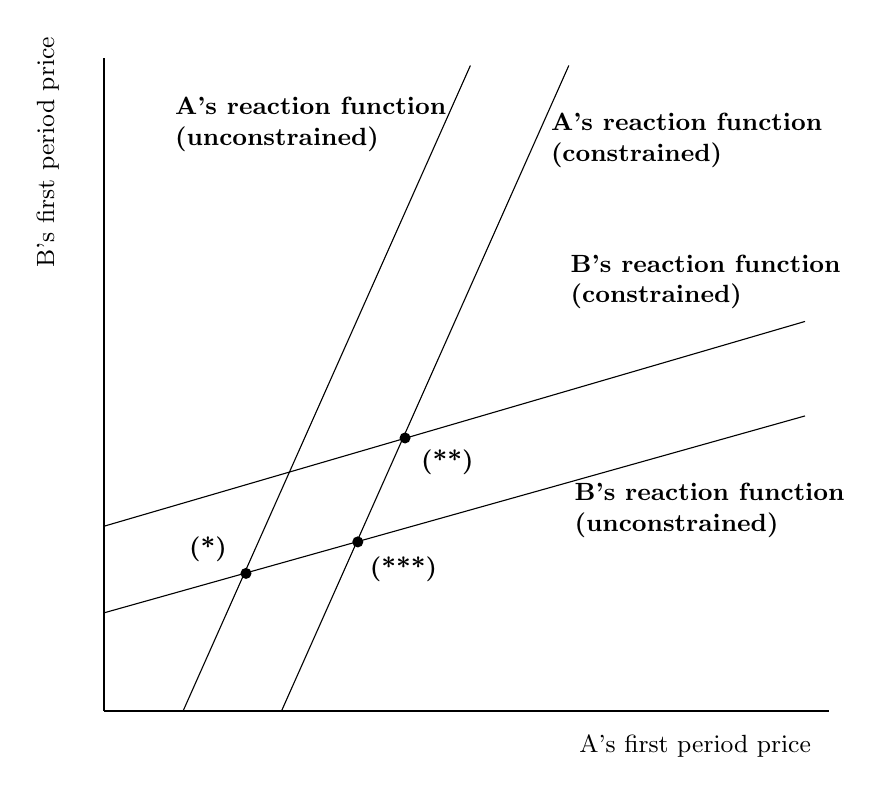
\begin{tikzpicture}[
    x=1cm,
    y=1cm,
    >=stealth,
    every node/.style={font=\small}
]

% Axes
\draw[thick] (0,0) -- (0,8.3);
\draw[thick] (0,0) -- (9.2,0);

% Axis labels
\node[rotate=90, anchor=south] at (-0.45,7.1)
    {B's first period price};

\node[anchor=north east] at (9.1,-0.18)
    {A's first period price};

% ------------------------------------------------
% A's reaction functions: steep lines
% ------------------------------------------------

% A constrained
\draw (1.0,0) -- (4.65,8.2);

% A unconstrained
\draw (2.25,0) -- (5.90,8.2);

% ------------------------------------------------
% B's reaction functions: shallow lines
% ------------------------------------------------

% B constrained
\draw (0,2.35) -- (8.9,4.95);

% B unconstrained
\draw (0,1.25) -- (8.9,3.75);

% ------------------------------------------------
% Labels
% ------------------------------------------------

\node[align=left, anchor=west] at (0.775,7.45)
{
    \textbf{A's reaction function}\\
    \textbf{(unconstrained)}
};

\node[align=left, anchor=west] at (5.55,7.25)
{
    \textbf{A's reaction function}\\
    \textbf{(constrained)}
};

\node[align=left, anchor=west] at (5.80,5.45)
{
    \textbf{B's reaction function}\\
    \textbf{(constrained)}
};

\node[align=left, anchor=west] at (5.85,2.55)
{
    \textbf{B's reaction function}\\
    \textbf{(unconstrained)}
};

% ------------------------------------------------
% Intersection points
% ------------------------------------------------

% (*)
\fill (1.80,1.75) circle (2pt);
\node[anchor=south east] at (1.68,1.78)
    {\textbf{(*)}};

% (**)
\fill (3.82,3.47) circle (2pt);
\node[anchor=north west] at (3.90,3.44)
    {\textbf{(**)}};

% (***)
\fill (3.22,2.15) circle (2pt);
\node[anchor=north west] at (3.25,2.08)
    {\textbf{(***)}};

\end{tikzpicture}
